\documentclass[11pt,a4paper]{article}

\usepackage[utf8]{inputenc}
\usepackage[T1]{fontenc}
\usepackage[french]{babel}
\usepackage[margin=2.2cm]{geometry}
\usepackage{graphicx}
\usepackage{float}
\usepackage{xcolor}
\usepackage{listings}
\usepackage{booktabs}
\usepackage{hyperref}

\hypersetup{colorlinks=true, linkcolor=blue!50!black, urlcolor=blue!60!black}
\graphicspath{{captures/}}

\definecolor{fond}{RGB}{245,245,245}
\definecolor{titreRouge}{RGB}{180,30,30}
\definecolor{qstVert}{RGB}{0,120,60}

% Grands titres en rouge
\makeatletter
\renewcommand\section{\@startsection{section}{1}{\z@}%
  {-3.5ex \@plus -1ex \@minus -.2ex}%
  {2.3ex \@plus.2ex}%
  {\normalfont\Large\bfseries\color{titreRouge}}}
\renewcommand\subsection{\@startsection{subsection}{2}{\z@}%
  {-3.25ex\@plus -1ex \@minus -.2ex}%
  {1.5ex \@plus .2ex}%
  {\normalfont\large\bfseries\color{titreRouge}}}
\makeatother

\lstset{
  basicstyle=\ttfamily\small,
  backgroundcolor=\color{fond},
  frame=single,
  rulecolor=\color{gray!50},
  breaklines=true,
  columns=fullflexible,
  keepspaces=true,
  showstringspaces=false,
  literate={é}{{\'e}}1 {è}{{\`e}}1 {à}{{\`a}}1 {ç}{{\c{c}}}1 {ê}{{\^e}}1 {É}{{\'E}}1
}
\lstdefinestyle{yaml}{language=, morecomment=[l]{\#}, commentstyle=\color{gray}}

% Questions en vert, réponses en texte normal (pas de bulle)
\newenvironment{reponse}[1]{%
  \par\medskip
  \noindent{\bfseries\color{qstVert}#1}\par\smallskip
  \noindent\ignorespaces
}{%
  \par\medskip
}

\title{\textbf{TP Kubernetes : déployer une stack ML « Breast Cancer »}\\[0.4em]
\large Compte rendu -- Parties A et B}
\author{Sabrine ESSADEQ\\ Cloud \& IA -- FSSM\\ Encadrant : Pr. Mohammed AMEKSA}
\date{\today}

\begin{document}

% Page 1 : uniquement la page de titre
\begin{titlepage}
  \centering
  \vspace*{3.5cm}
  {\LARGE\bfseries TP Kubernetes : déployer une stack ML « Breast Cancer »\par}
  \vspace{1.2cm}
  {\Large Compte rendu -- Parties A et B\par}
  \vspace{2.5cm}
  {\large Sabrine ESSADEQ\par}
  \vspace{0.6cm}
  {\large Cloud \& IA -- FSSM\par}
  \vspace{0.4cm}
  {\large Encadrant : Pr. Mohammed AMEKSA\par}
  \vfill
  {\large \today\par}
\end{titlepage}

% Page 2 : table des matières
\tableofcontents
\newpage

%=====================================================================
\section{Introduction}
%=====================================================================
Dans ce TP, j'ai déployé sur Minikube une application de Machine Learning
autour du jeu de données \emph{Breast Cancer Wisconsin} (569 tumeurs, 30 mesures) :
\begin{itemize}
  \item une \textbf{classification} : la tumeur est-elle maligne ou bénigne ?
  \item une \textbf{régression} : prédire la surface moyenne (\texttt{mean area}) à partir des 29 autres mesures.
\end{itemize}

Le code et les Dockerfiles étaient fournis. J'ai écrit tous les manifestes
Kubernetes (dossier \texttt{k8s/}) avec la méthode \textbf{GMA} :
\textbf{G}énérer le squelette (\texttt{--dry-run=client -o yaml}),
\textbf{M}odifier le fichier, \textbf{A}ppliquer (\texttt{kubectl apply -f}).

\subsection*{Architecture cible}
\begin{center}
\begin{tabular}{lll}
\toprule
Composant & Rôle & Objets Kubernetes \\
\midrule
Job \texttt{bc-train-v1} & Entraîne les 2 modèles et les dépose dans MinIO & Job \\
\texttt{minio} & Stockage objet S3 des modèles (bucket \texttt{models}) & Deployment, Service, Secret \\
\texttt{redis} & Compteur et cache des prédictions & Deployment, Service \texttt{base} \\
\texttt{bc-api} & API FastAPI de prédiction & Deployment, Service, ConfigMap, Secret \\
\texttt{bc-front} & Interface Streamlit & Deployment, Service \\
\texttt{bc-ingress} & Point d'entrée HTTP \texttt{bc.local} & Ingress \\
\bottomrule
\end{tabular}
\end{center}

Le navigateur n'entre que par l'Ingress ; le front appelle l'API en interne par le nom
de son Service, et l'API retrouve MinIO et Redis de la même façon.

%=====================================================================
\section{Préparation de l'environnement}
%=====================================================================

\subsection{Démarrage du cluster Minikube}
Minikube crée un cluster Kubernetes d'un seul nœud, exécuté dans un conteneur Docker
(driver \texttt{docker}). Au premier lancement, il télécharge l'image de base du nœud
(\texttt{kicbase}) et les composants préchargés de Kubernetes.

\begin{lstlisting}
minikube start --driver=docker
\end{lstlisting}

\begin{figure}[H]
  \centering
  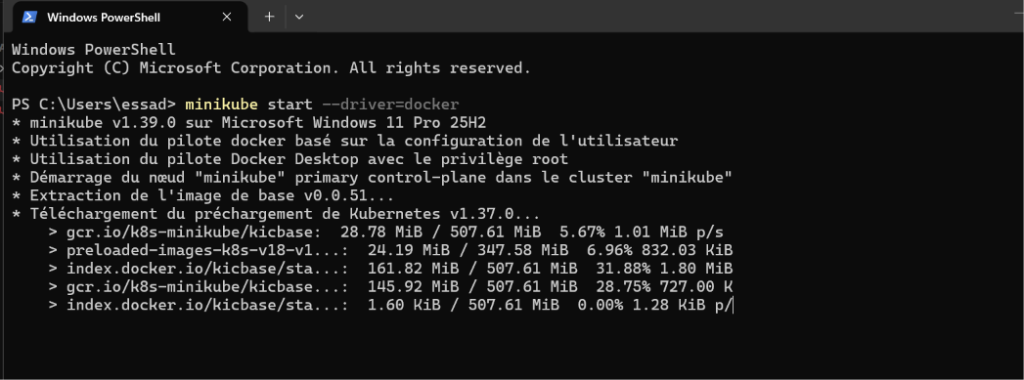
\includegraphics[width=0.9\linewidth]{00-minikube-start.png}
  \caption{Premier démarrage de Minikube : téléchargement de l'image du nœud et de Kubernetes v1.37.}
\end{figure}

Les addons \texttt{ingress} (contrôleur nginx) et \texttt{metrics-server} (métriques CPU/mémoire)
sont ensuite activés. Le nœud doit être \texttt{Ready}.

\begin{lstlisting}
minikube addons enable ingress
minikube addons enable metrics-server
kubectl get nodes
minikube addons list | findstr "ingress metrics"
\end{lstlisting}

\begin{figure}[H]
  \centering
  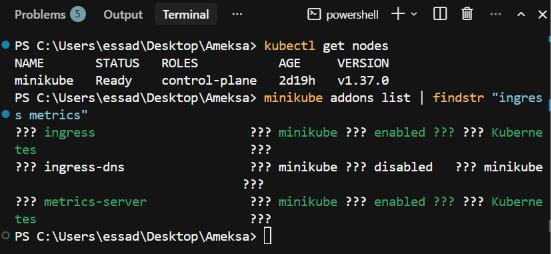
\includegraphics[width=0.95\linewidth]{00-cluster.png}
  \caption{Cluster Minikube prêt : nœud Ready, addons ingress et metrics-server activés.}
\end{figure}

\subsection{Variables d'environnement lues par l'API}
La lecture de \texttt{app/api/main.py} montre que toute la configuration de l'API est
lue par \texttt{os.getenv(...)}. Chaque variable est fournie par une source différente
selon sa nature :

\begin{center}
\small
\begin{tabular}{lll}
\toprule
Variable & Source dans Kubernetes & Justification \\
\midrule
\texttt{MINIO\_ACCESS\_KEY}, \texttt{MINIO\_SECRET\_KEY} & Secret \texttt{minio-secret} & identifiants sensibles \\
\texttt{API\_KEY} & Secret \texttt{api-secret} & clé d'accès sensible \\
\texttt{MINIO\_ENDPOINT}, \texttt{MINIO\_BUCKET} & ConfigMap \texttt{ml-config} & configuration non sensible \\
\texttt{REDIS\_HOST}, \texttt{REDIS\_PORT} & ConfigMap \texttt{ml-config} & configuration non sensible \\
\texttt{CACHE\_TTL}, \texttt{LOG\_LEVEL} & ConfigMap \texttt{ml-config} & réglages de fonctionnement \\
\texttt{MODEL\_VERSION} & \texttt{env} du Deployment & liée à la version déployée \\
\texttt{APP\_VERSION} & image (\texttt{ARG}/\texttt{ENV} du Dockerfile) & gravée au build \\
\texttt{MODEL\_CONFIG\_PATH} & valeur par défaut & chemin du ConfigMap \texttt{model-config} monté \\
\bottomrule
\end{tabular}
\end{center}

\subsection{Construction des images et dossier \texttt{k8s/}}
Les images sont construites localement puis chargées dans Minikube
(\texttt{minikube image load}), car le stockage d'images de Minikube est distinct
de celui de Docker Desktop.

\begin{lstlisting}
cd "C:\Users\essad\Desktop\Ameksa\tp ml-k8s"
mkdir k8s
Set-ExecutionPolicy -Scope Process -ExecutionPolicy Bypass
.\scripts\build-images.ps1
minikube image ls | findstr bc-
\end{lstlisting}

\begin{figure}[H]
  \centering
  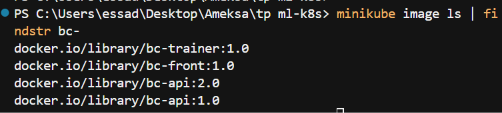
\includegraphics[width=0.95\linewidth]{00-images.png}
  \caption{Les quatre images \texttt{bc-*} présentes dans Minikube.}
\end{figure}

\begin{reponse}{Q1 -- Pourquoi \texttt{minikube image load} ?}
Quand je fais \texttt{docker build}, l'image se retrouve dans Docker Desktop.
Minikube a son propre stockage d'images dans le nœud, donc il ne la voit pas
automatiquement. Il faut la copier avec \texttt{minikube image load}.

Avec \texttt{imagePullPolicy: Always}, Kubernetes essaierait de télécharger
l'image depuis Internet. Or mes images \texttt{bc-*} n'y sont pas publiées,
donc le Pod resterait bloqué en \texttt{ErrImagePull} /
\texttt{ImagePullBackOff}. C'est pour ça que j'utilise \texttt{IfNotPresent}.
\end{reponse}

\begin{reponse}{Q2 -- Différence entre \texttt{bc-api:1.0} et \texttt{bc-api:2.0}}
En regardant le Dockerfile de l'API, je vois que le code est le même.
Ce qui change, c'est juste \texttt{APP\_VERSION}, passée au build avec
\texttt{--build-arg} et enregistrée dans l'image (\texttt{ARG}/\texttt{ENV}).
\end{reponse}

%=====================================================================
\section{Un Pod seul, et ses limites}
%=====================================================================

\subsection{Méthode GMA}
\begin{lstlisting}
kubectl run bc-api-pod --image=bc-api:1.0 --image-pull-policy=IfNotPresent --port=8000 --dry-run=client -o yaml > k8s/00-pod-api.yaml
kubectl apply -f k8s/00-pod-api.yaml
kubectl get pods -o wide
kubectl logs bc-api-pod
\end{lstlisting}

Le Pod passe en \texttt{1/1 Running} : le serveur Uvicorn démarre. Les logs montrent
cependant des erreurs répétées \texttt{Failed to resolve 'minio'} et
\texttt{modèles v1 indisponibles} : aucun MinIO n'est encore déployé.

\begin{lstlisting}
kubectl delete pod bc-api-pod
kubectl get pods
# No resources found in default namespace.
\end{lstlisting}

\begin{reponse}{Q3 -- Running mais capable de prédire ?}
Non. Le Pod est en \texttt{1/1 Running}, donc le conteneur a démarré, mais
dans les logs je vois \texttt{Failed to resolve 'minio'} et
\texttt{modèles v1 indisponibles}. Sans MinIO ni modèles, l'API ne peut
pas prédire.
\end{reponse}

\begin{reponse}{Q4 -- Le Pod revient-il après suppression ?}
Non. Après \texttt{kubectl delete pod bc-api-pod}, j'obtiens
\texttt{No resources found}. Un Pod seul n'est pas géré par un contrôleur.
Il faut un Deployment pour qu'il soit recréé automatiquement.
\end{reponse}

%=====================================================================
\section{Secrets et ConfigMaps}
%=====================================================================

On externalise la configuration : rien de sensible dans les images.
Méthode GMA (\texttt{--dry-run=client -o yaml}), puis \texttt{kubectl apply -f}.

\begin{lstlisting}
kubectl apply -f k8s/01-secrets.yaml
kubectl apply -f k8s/02-configmaps.yaml
kubectl get cm,secret
kubectl describe cm ml-config
\end{lstlisting}

Résultat : Secrets \texttt{minio-secret} (2 clés) et \texttt{api-secret} (1 clé) ;
ConfigMaps \texttt{ml-config} (7 variables) et \texttt{model-config} (fichier
\texttt{threshold\_malin: 0.5}).

\begin{reponse}{Q5 -- Un Secret est-il chiffré ?}
Pas vraiment : c'est du Base64, je peux le décoder facilement. Donc je ne
dois pas mettre \texttt{01-secrets.yaml} sur un Git public, et je fais
attention aux droits d'accès.
\end{reponse}

\begin{reponse}{Q6 -- Pourquoi \texttt{"6379"} entre guillemets ?}
Parce qu'en YAML, sans guillemets, 6379 serait un nombre. Un ConfigMap
n'accepte que des chaînes. Avec \texttt{"6379"}, c'est clairement du texte.
\end{reponse}

%=====================================================================
\section{MinIO, le stockage des modèles}
%=====================================================================

MinIO stocke les modèles (API S3). Deployment + Service \texttt{minio:9000}
(API) et \texttt{9001} (console). Identifiants lus depuis \texttt{minio-secret}
via \texttt{secretKeyRef}. Volume \texttt{emptyDir} sur \texttt{/data},
stratégie \texttt{Recreate}.

\begin{lstlisting}
kubectl apply -f k8s/03-minio.yaml
kubectl port-forward svc/minio 9001:9001
# navigateur : http://localhost:9001  (tpadmin / Tp-M1ni0-2026!)
\end{lstlisting}

\begin{figure}[H]
  \centering
  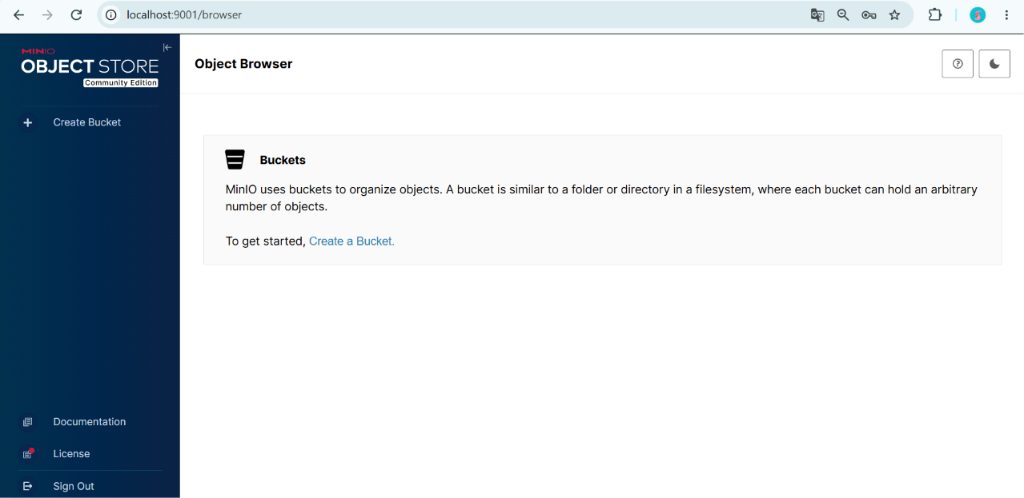
\includegraphics[width=0.85\linewidth]{03-minio.png}
  \caption{Console MinIO : connectée, aucun bucket (créé plus tard par le Job).}
\end{figure}

\begin{reponse}{Q7 -- Noms différents Secret / variables MinIO}
MinIO attend \texttt{MINIO\_ROOT\_USER} / \texttt{MINIO\_ROOT\_PASSWORD},
alors que mon Secret a \texttt{MINIO\_ACCESS\_KEY} /
\texttt{MINIO\_SECRET\_KEY}. Je fais le lien avec
\texttt{valueFrom.secretKeyRef} : je choisis le nom de la variable du
conteneur et je pointe vers la clé du Secret.
\end{reponse}

\begin{reponse}{Q8 -- Que deviennent les modèles si le Pod MinIO est supprimé ?}
Avec \texttt{emptyDir}, les modèles sont perdus si le Pod MinIO est
supprimé. Pour les garder, il faudrait un PersistentVolumeClaim (PVC).
\end{reponse}

%=====================================================================
\section{Le Job d'entraînement v1}
%=====================================================================

Job \texttt{bc-train-v1} : image \texttt{bc-trainer:1.0},
\texttt{MODEL\_VERSION=v1}, \texttt{ALGO=linear},
\texttt{backoffLimit: 4}, \texttt{restartPolicy: Never}.

\begin{lstlisting}
kubectl apply -f k8s/04-train-job-v1.yaml
kubectl logs job/bc-train-v1
\end{lstlisting}

Le Pod passe en \texttt{Completed}. Les modèles sont déposés dans
\texttt{s3://models/v1/} (3 fichiers).

\begin{reponse}{Q9 -- Métriques relevées}
J'ai relevé : accuracy = 0,9825 et F1 = 0,9861 (classification) ;
R² = 0,9952 et MAE = 15,37 (régression).
L'accuracy est le \% de bons diagnostics ; le F1 mélange précision et
rappel. Le R² mesure la qualité de la régression ; la MAE est l'erreur
moyenne absolue.
\end{reponse}

\begin{reponse}{Q10 -- Pourquoi un Job ? restartPolicy ? re-apply ?}
J'utilise un Job parce que l'entraînement doit se terminer puis
s'arrêter. Un Deployment garderait des Pods allumés en permanence.
\texttt{restartPolicy: Always} est interdit dans un Job.
Si je refais \texttt{kubectl apply} sur le même Job, rien ne se
relance : pour réentraîner, je dois le supprimer puis le recréer.
\end{reponse}

%=====================================================================
\section{Redis, la « base »}
%=====================================================================

Deployment \texttt{redis} (image \texttt{redis:7-alpine}) + Service ClusterIP
nommé \texttt{base}. Test : \texttt{redis-cli ping} $\rightarrow$ \texttt{PONG},
et \texttt{nslookup base} résout \texttt{base.default.svc.cluster.local}.

\begin{reponse}{Q11 -- redis vs base}
L'API utilise le nom du Service \texttt{base}, configuré dans
\texttt{ml-config} (\texttt{REDIS\_HOST=base}). Le Deployment
s'appelle \texttt{redis}, mais c'est le nom du Service qui compte
pour le DNS.
\end{reponse}

%=====================================================================
\section{L'API de prédiction}
%=====================================================================

Deployment \texttt{bc-api} avec 3 réplicas, image \texttt{bc-api:1.0},
ConfigMap + Secrets, volume \texttt{model-config}, Service sur le port 8000.
Les logs confirment : \texttt{modèles v1 chargés depuis s3://models/v1/}.
Le script \texttt{test-api.ps1} a validé classification (\texttt{malin})
et régression (\texttt{mean area}).

%=====================================================================
\section{Frontend et Ingress}
%=====================================================================

Deployment \texttt{bc-front} (Streamlit) + Service port 80~$\rightarrow$~8501.
Ingress \texttt{bc-ingress} : hôte \texttt{bc.local}, \texttt{/api} vers
l'API, \texttt{/} vers le front. Accès Windows : \texttt{minikube tunnel}
+ entrée \texttt{127.0.0.1 bc.local} dans le fichier \texttt{hosts}.

\begin{figure}[H]
  \centering
  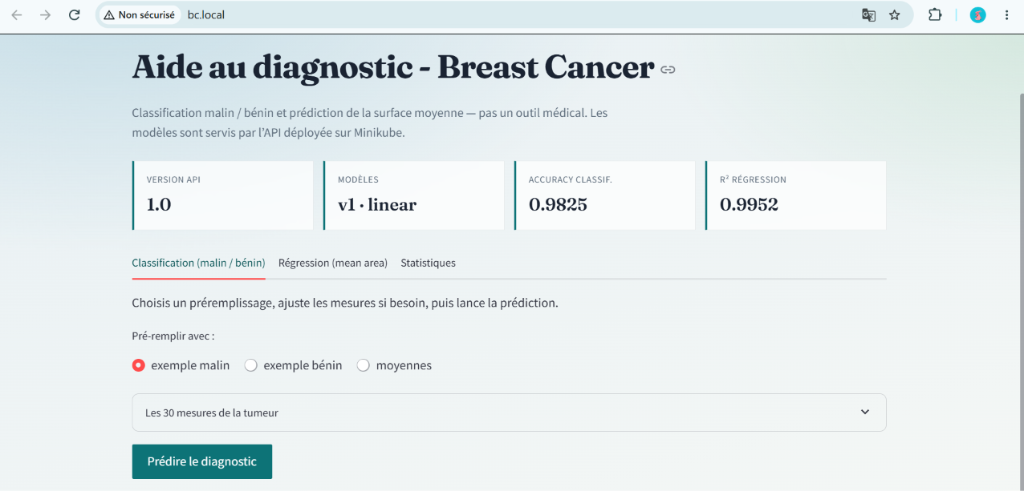
\includegraphics[width=0.92\linewidth]{08-bc-local.png}
  \caption{Interface \texttt{http://bc.local} : modèles v1 (linear).}
\end{figure}

\begin{figure}[H]
  \centering
  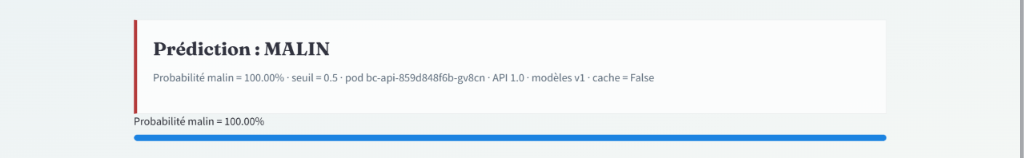
\includegraphics[width=0.92\linewidth]{08-prediction-malin.png}
  \caption{Classification sur l'exemple malin (prédiction MALIN).}
\end{figure}

\begin{reponse}{Q12 -- Pourquoi \texttt{http://bc-api:8000} et pas \texttt{bc.local/api} ?}
Parce que le front appelle l'API en interne par le nom du Service.
Ça reste dans le cluster, ça ne dépend pas du tunnel / hosts, et
\texttt{bc.local} sert surtout à mon navigateur.
\end{reponse}

\begin{reponse}{Q13 -- Comment l'Ingress choisit \texttt{/api/info} ?}
Les deux règles commencent par \texttt{/}, mais Nginx prend la plus
spécifique. \texttt{/api} matche \texttt{/api/info} donc ça va vers
l'API ; le reste va vers le front.
\end{reponse}

%=====================================================================
\section{État final de la partie A}
%=====================================================================

Objectif atteint : \texttt{http://bc.local} prédit avec les modèles v1.
Ressources principales : Deployments \texttt{minio}, \texttt{redis},
\texttt{bc-api} (3), \texttt{bc-front} ; Services \texttt{minio},
\texttt{base}, \texttt{bc-api}, \texttt{bc-front} ; Job
\texttt{bc-train-v1} Completed ; Ingress \texttt{bc-ingress} ;
ConfigMaps / Secrets.

\begin{lstlisting}
kubectl get deploy,svc,ingress,jobs,cm,secret
\end{lstlisting}

\begin{figure}[H]
  \centering
  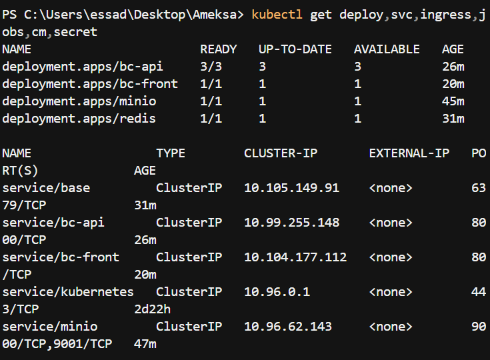
\includegraphics[width=0.95\linewidth]{08-final-1.png}
  \caption{État final (1/2) : Deployments et Services.}
\end{figure}

\begin{figure}[H]
  \centering
  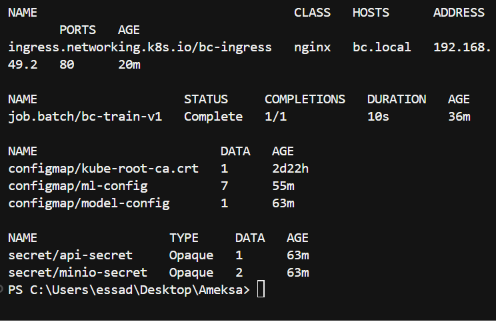
\includegraphics[width=0.95\linewidth]{08-final-2.png}
  \caption{État final (2/2) : Ingress, Job, ConfigMaps et Secrets.}
\end{figure}

\newpage
%=====================================================================
\section{Partie B -- Sondes et ressources}
%=====================================================================

Ajout des sondes startup / liveness / readiness et des
requests/limits sur \texttt{bc-api}, \texttt{bc-front}, \texttt{minio}
et \texttt{redis}.

\begin{reponse}{Q14 -- Les trois sondes}
Startup (\texttt{/health}) : l'API a-t-elle fini de démarrer ?
Sinon Kubernetes attend.
Liveness (\texttt{/health}) : est-elle encore vivante ?
Sinon Kubernetes redémarre le conteneur.
Readiness (\texttt{/ready}) : peut-elle recevoir du trafic ?
Sinon le Pod est retiré du Service, sans restart.
\end{reponse}

\begin{reponse}{Q15 -- Expérience A (Redis arrêté)}
Non, je n'ai pas vu de restart : les Pods API étaient en
\texttt{0/1 Running} avec RESTARTS à 0. C'est normal : Redis down
ne veut pas dire que l'API est morte, elle ne doit juste plus
recevoir de trafic. Si la liveness était sur \texttt{/ready},
Kubernetes redémarrerait les Pods en boucle.
\end{reponse}

\begin{reponse}{Q16 -- Délai avant restart (Exp B)}
Environ 30~s : $3 \times 10$ (\texttt{failureThreshold} $\times$
\texttt{periodSeconds}). J'ai vu dans les Events
\texttt{Liveness probe failed} puis le restart du conteneur.
\end{reponse}

\begin{reponse}{Q17 -- Startup plus longue sur le front}
Parce que Streamlit démarre plus lentement. Sans startupProbe,
la liveness pourrait tuer le Pod trop tôt.
\end{reponse}

%=====================================================================
\section{Partie B -- Configuration à chaud}
%=====================================================================

Passage de \texttt{threshold\_malin} de 0,5 à 0,05 dans le ConfigMap
monté en fichier : le Pod voit la nouvelle valeur sans restart.
Exemple bénin (proba $\approx$ 8,5~\%) devient \textbf{malin} avec
le seuil 0,05.

\begin{reponse}{Q18 -- Fichier vs variable d'environnement}
J'ai vu le nouveau seuil dans le fichier après environ une minute,
sans redémarrer les Pods. \texttt{LOG\_LEVEL} n'a changé qu'après
\texttt{rollout restart}, parce qu'une variable d'environnement
est figée au démarrage.
\end{reponse}

\begin{reponse}{Q19 -- Pourquoi pas \texttt{subPath} ?}
Avec \texttt{subPath}, le fichier est collé une fois au démarrage
et ne se met plus à jour. Sans \texttt{subPath}, il peut changer
quand le ConfigMap change.
\end{reponse}

\begin{reponse}{Q20 -- Seuil bas (point de vue médical)}
Avec un seuil bas, je détecte plus de cas suspects (moins de faux
négatifs) mais j'augmente les fausses alertes (plus de faux
positifs).
\end{reponse}

%=====================================================================
\section{Partie B -- HPA et mise à jour v2 / rollback}
%=====================================================================

Scaling manuel à 5 puis retour à 3. HPA \texttt{bc-api} : min 2,
max 6, cible CPU 50~\%. Job \texttt{bc-train-v2} (algo forest),
puis rolling update vers \texttt{bc-api:2.0} + \texttt{MODEL\_VERSION=v2},
enfin \texttt{rollout undo}.

\begin{center}
\begin{tabular}{lcc}
\toprule
Métrique & v1 linear & v2 forest \\
\midrule
accuracy & 0,9825 & 0,9561 \\
F1 & 0,9861 & 0,9655 \\
R² & 0,9952 & 0,9981 \\
MAE & 15,37 & 7,69 \\
\bottomrule
\end{tabular}
\end{center}

\begin{reponse}{Q21 -- Rolling update sans coupure}
Pendant la mise à jour, j'ai surtout vu \texttt{1.0 v1} puis
\texttt{2.0 v2}, sans vraiment d'erreurs. Grâce à
\texttt{maxSurge: 1} et \texttt{maxUnavailable: 0}, un nouveau Pod
est créé et ready avant de retirer un ancien. La readiness évite
d'envoyer du trafic trop tôt.
\end{reponse}

\begin{reponse}{Q22 -- Quelle version garder ?}
\begin{center}
\begin{tabular}{lcc}
\toprule
 & v1 linear & v2 forest \\
\midrule
accuracy & 0,9825 & 0,9561 \\
F1 & 0,9861 & 0,9655 \\
R² & 0,9952 & 0,9981 \\
MAE & 15,37 & 7,69 \\
\bottomrule
\end{tabular}
\end{center}
Pour la classification je garde la v1. Pour la régression, la v2.
Je proposerais de garder le meilleur modèle pour chaque tâche.
\end{reponse}

\begin{reponse}{Q23 -- MODEL\_VERSION dans le Deployment}
Parce qu'elle doit changer avec l'image. Dans le Deployment, le
\texttt{rollout undo} remet les deux. Si elle était dans le
ConfigMap, je me retrouverais avec l'image v1 et les modèles v2.
\end{reponse}

\begin{reponse}{Q24 -- ReplicaSets après rollback}
J'en vois plusieurs. Celui de la v1 a DESIRED=3 (Pods actifs).
Celui de la v2 a DESIRED=0 mais reste grâce à
\texttt{revisionHistoryLimit}, pour l'historique / un éventuel redo.
\end{reponse}

%=====================================================================
\section{Conclusion}
%=====================================================================

J'ai déployé la stack jusqu'à \texttt{http://bc.local} (partie A),
puis j'ai ajouté les sondes, le HPA, la config à chaud et le
rolling update / rollback (partie B).

\end{document}
